\begin{flushright} {\tiny {\color{gray} (tikz\_han.tex)}} \end{flushright}
%~~~~~~~~~~~~~~~~~~~~~~~~~~~~~~~~~~~~~~~~~~~~~~~~~~~~~~~~~~~~~~~~~~~~~~~~~~~~~~~~~~~~~~~~~~~~~~~~~~



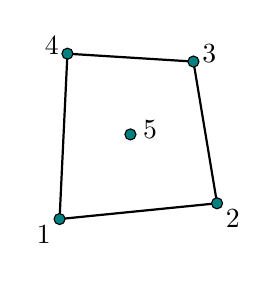
\begin{tikzpicture}
%\draw[fill=gray!23,gray!23](0,0) rectangle (5,5);
%\draw[step=0.5cm,gray,very thin] (0,0) grid (4,4); %background grid
\draw[thick] (1,1) -- (3,1.2) -- (2.7,3) -- (1.1,3.1) -- cycle;  
\node[] at (0.8,0.8) {1};
\node[] at (3.2,1) {2};
\node[] at (2.9,3.1) {3};
\node[] at (0.9,3.2) {4};
\node[] at (2.15,2.13) {5};
\draw[black,fill=teal] (1.9,2.075) circle (2pt);
\draw[black,fill=teal] (1,1)   circle (2pt);
\draw[black,fill=teal] (3,1.2)  circle (2pt);
\draw[black,fill=teal] (2.7,3)  circle (2pt);
\draw[black,fill=teal] (1.1,3.1) circle (2pt);
\end{tikzpicture}


